../cictikz/src/cictikz/data/tex/cictikz_preamble.tex

% The research universe, redrawn from the hand-painted original
% (media/education.pdf): concentric territories from Easy at the
% centre out through Complicated, Possible and Unknown, with the
% Impossible beyond the last ring. The rings are drawn slightly
% wobbly on purpose - the borders of knowledge are not circles.

\definecolor{uEasy}{RGB}{58,122,110}
\definecolor{uCompl}{RGB}{190,196,130}
\definecolor{uPoss}{RGB}{214,158,80}
\definecolor{uUnkn}{RGB}{110,105,100}

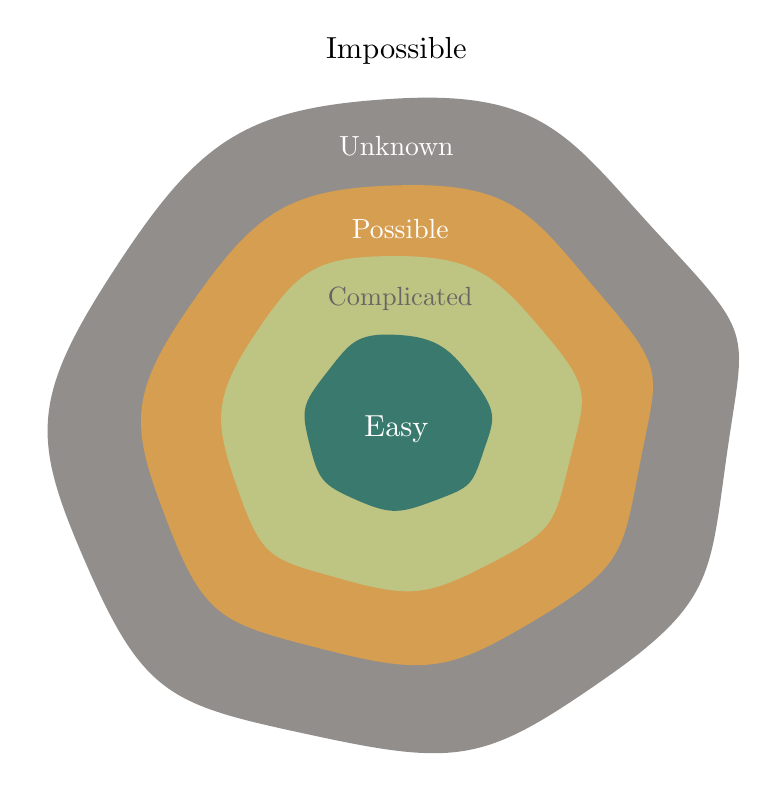
\begin{tikzpicture}[thick]

  % ---- unknown ----
  \fill[uUnkn!75] plot[smooth cycle, tension=1]
    coordinates {(0,4.1) (3.4,2.3) (4.2,-0.4) (2.6,-3.3) (-1.0,-4.0) (-3.9,-1.9) (-3.6,1.9)};
  % ---- possible ----
  \fill[uPoss] plot[smooth cycle, tension=1]
    coordinates {(0.1,3.0) (2.6,1.6) (3.1,-0.5) (1.8,-2.5) (-0.9,-2.9) (-2.9,-1.3) (-2.6,1.5)};
  % ---- complicated ----
  \fill[uCompl] plot[smooth cycle, tension=1]
    coordinates {(0.0,2.1) (1.9,1.1) (2.2,-0.5) (1.2,-1.8) (-0.7,-2.0) (-2.0,-0.9) (-1.8,1.1)};
  % ---- easy ----
  \fill[uEasy] plot[smooth cycle, tension=1]
    coordinates {(0.0,1.1) (1.0,0.5) (1.1,-0.4) (0.5,-1.0) (-0.5,-1.0) (-1.1,-0.3) (-0.9,0.6)};

  % ---- labels ----
  \node[anchor=center, scale=1.1] at (0,4.7) {Impossible};
  \node[white, anchor=center] at (0,3.5) {Unknown};
  \node[white, anchor=center] at (0.05,2.45) {Possible};
  \node[black!60, anchor=center, scale=0.95] at (0.05,1.55) {Complicated};
  \node[white, anchor=center, scale=1.1] at (0,-0.1) {Easy};

\end{tikzpicture}
\end{document}
